\newpage
\section{\productNameMed{} Integration} 
\label{sec:monitor_program}

As we mentioned earlier, the {\it \systemNameFull} system, and the sample programs described
in this document, are made available as part of the \productNameMed{}. Figures
\ref{fig:monitor_project} to
\ref{fig:monitor_last} show a series of windows that are used in the Monitor 
Program to create a new project.
In the first screen, shown in Figure \ref{fig:monitor_project}, the user specifies a 
file system folder where the
project will be stored, gives the project a name, and specifies the type of processor that
is being used. Pressing {\sf Next} opens the window
in Figure \ref{fig:monitor_system}. Here, the user can select the {\it \systemNameFull} 
as a pre-designed system.
The Monitor Program then fills in the relevant information in the {\it System details} box,
which includes the appropriate system info and FPGA configuration files, and preloader.
The first of these files specifies to the Monitor Program information about the components 
that are available in the {\it \systemNameFull}, such as the type of processor and memory 
components, and the address map. The second file is an FPGA programming bitstream for 
the {\it \systemNameFull}, which can downloaded by the Monitor Program into the \DEBoard~board. 
Any system which contains a Hard Processor System (HPS) component must also specify the preloader to be
run immediately following the circuit being downloaded. This preloader is used to configure the components
within the HPS with the setting required for the specific board.
~\\
~\\
\begin{figure}[h!]
	\centering
	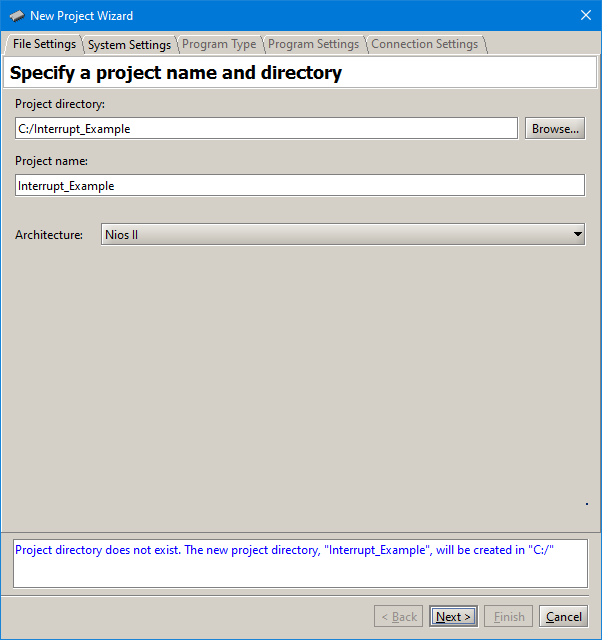
\includegraphics[scale=0.65]{figures/fig_monitor_project.png}
	\caption{Specifying the project folder and project name.}
	\label{fig:monitor_project}
\end{figure}

\clearpage
\newpage
Pressing {\sf Next} again opens the window in Figure \ref{fig:monitor_samples}. Here the
user selects the type of program that will be used, such as Assembly language, or C. Then,
the check box shown in the figure can be used to display the list of sample programs for
the {\it \systemNameFull} that are described in this document. When a sample program
is selected in this list, its source files, and other settings, can be copied into the 
project folder in subsequent screens of the Monitor Program.

Figure \ref{fig:monitor_last} gives the final screen that is 
used to create a new project in the Monitor Program. This screen shows the default addresses of 
compiler and linker sections that will be used for the assembly language or C program 
associated with the Monitor Program project.  In the figure, the drop-down menu called 
{\it Linker Section Presets} has been set to {\sf Exceptions}. With this setting the 
Monitor Program uses specific compiler and linker sections for the selected processor.
For the \processor processor, these sections are for reset and
trap handler, and another section for the main program, called .{\it text}. For the
A9 processor, it has a section for the exception table, 
called .{\it vectors}, and another section
for the main program, called .{\it text}. It also shows the initial value used to set the main 
stack pointer for C programs, which is the starting address of the .{\it stack} section.
~\\
~\\
\begin{figure}[h!]
	\centering
	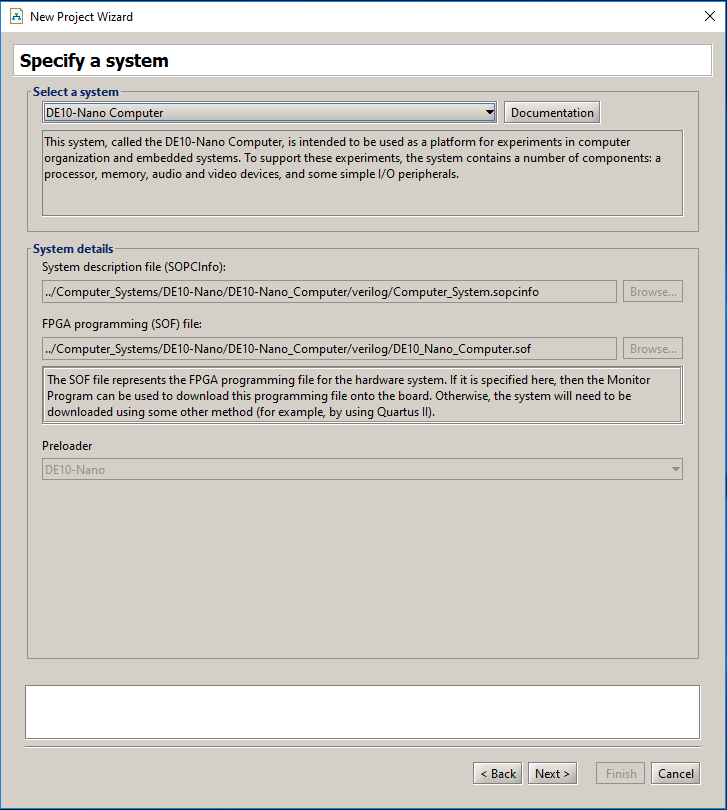
\includegraphics[scale=0.60]{figures/fig_monitor_system.png}
	\caption{Specifying the {\systemNameFull}.}
	\label{fig:monitor_system}
\end{figure}

\begin{figure}[h!]
	\centering
	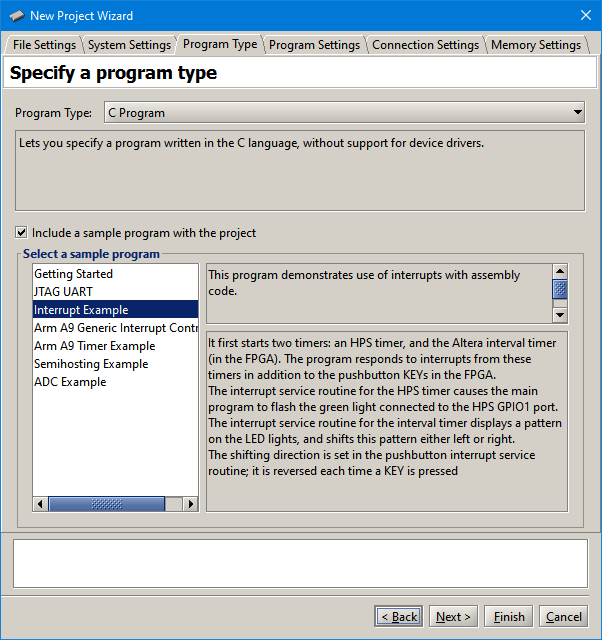
\includegraphics[scale=0.55]{figures/fig_monitor_samples.png}
	\caption{Selecting sample programs.}
	\label{fig:monitor_samples}
\end{figure}

\begin{figure}[h!]
\centering
	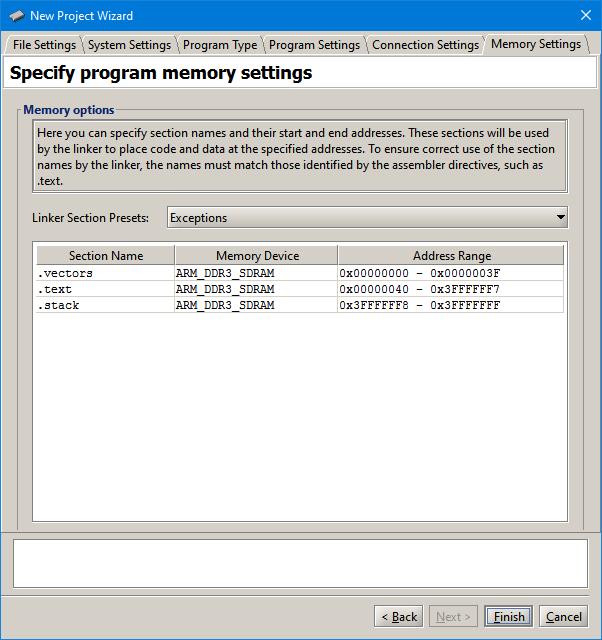
\includegraphics[scale=0.55]{figures/fig_monitor_last.png}
	\caption{Setting offsets for .{\it text} and .{\it data}.}
	\label{fig:monitor_last}
\end{figure}

